\documentclass[../TST.tex]{subfiles}
\begin{document}
\begin{pproblem}{\ }
Figure \ref{IV2} shows the I-V curve of a bulb. This bulb is connected in parallel with a resistance $R=\qty{2.00}{\ohm}$ to a source of EMF $E=\qty{15}{V}$ and internal resistance $r=\qty{3.00}{\ohm}$. Using the I-V curve, find the power $P$ dissipated in the bulb. Estimate the accuracy $\Delta P$ of your result.
\begin{figure}[h]
\centering
\hspace{-2em}
    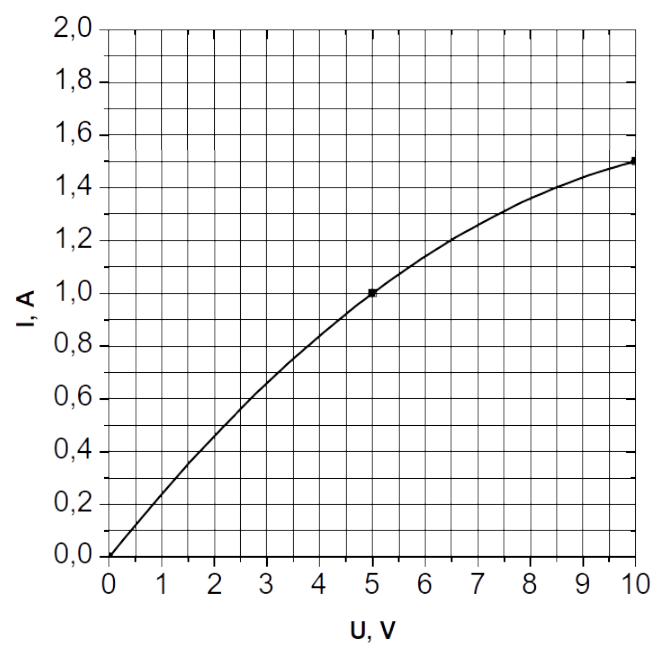
\includegraphics[width=0.5\textwidth]{fig/2007_s4.png}
    \caption{}
  \label{IV2}
\end{figure}
\end{pproblem}
\ifprob \else
	\begin{solution} Using Kirchhoff's rules, we will find a constraint on the state of the lightbulb $(U,I)$. Firstly, note that the voltage across the resistance $R$ is also $U$, and hence the current through it is $U/R$. Then, the total current through $r$ is $I+\frac{U}{R}$, and so the loop rule gives us
\begin{equation*}
	E- \left(I+\frac{U}{R}\right)r-U=0 \quad\Rightarrow\quad I=\frac{E}{r}-\frac{R+r}{Rr}U \quad\Rightarrow\quad I = \qty{5}{A} - (\qty{0.833}{\ohm^{-1}})\,U 
.
\end{equation*}
The voltage and the current of the lightbulb correspond to the point on the I-V curve which follows the constraint. On the graph, this constraint looks like a straight line. After we plot it and intersect it with the I-V curve, we estimate $U=\qty{4.8}{V}$ and $I=\qty{0.98}{A}$. Our results are very sensitive to the slope of the line, so we should have generous error estimates, e.g.\, $\Delta U=\qty{0.1}{V}$ and $\Delta I = \qty{0.02}{A}$. The dissipated power is $P=UI=\qty{4.704}{W}$, while the error in $P$ is
\begin{equation*}
\Delta P = \Delta (UI) = \Delta U I + U\Delta I= \qty{0.194}{W}
.
\end{equation*}
To present our answer properly, we need to round the error to one significant digit, and work with the same precision for $P$. Thus, \fbox{$P=\qty{4.7(0.2)}{W}$}.

\begin{center}
\hspace{-2em}
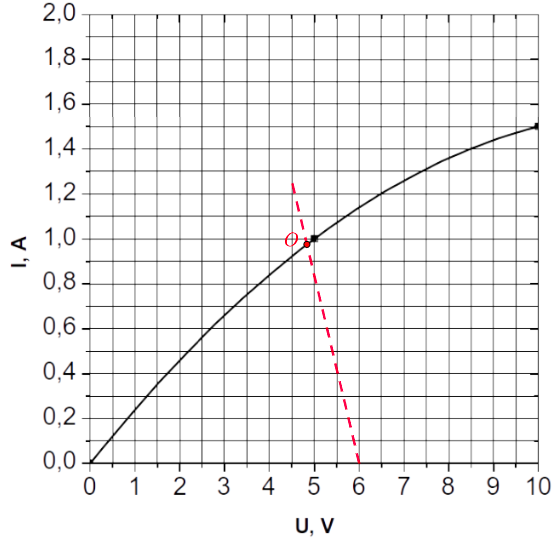
\includegraphics[width=0.5\textwidth]{fig/a2007_s4.png}
\end{center}

\end{solution}
\fi
\end{document}
